\documentclass{beamer}
\usetheme{Hannover}
\setbeamersize{sidebar width left=0pt}
\usepackage[T1, T2A]{fontenc}
\usepackage[utf8]{inputenc}
\usepackage[russian]{babel}
\usepackage{hyperref}
\usepackage{graphicx}
\graphicspath{ {../Images/} }

\author{Григорий Матюхин}
\date{\today}
\title{Лабораторная работа \textnumero15.}
\subtitle{Управление логическими томами}

\begin{document}
\begin{frame}[plain]
	\titlepage
\end{frame}
\section{Цель работы}
\begin{frame}[plain]
	\frametitle{Цель работы}
	Получить навыки управления логическими томами.
\end{frame}

\subsection{Создание физического тома}
\begin{enumerate}
	\begin{frame}[plain]
		\frametitle{Создание физического тома}
		\item В терминале с полномочиями администратора с помощью \texttt{fdisk} создайте основной раздел с типом LVM:
		\\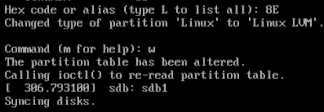
\includegraphics{4.png}
	\end{frame}
	\begin{frame}[plain]
		\item Обновите таблицу разделов:
		\item Теперь, когда раздел был создан, вы должны укажите его как физический том LVM:
		\item Убедитесь, что физический том создан успешно:
		\\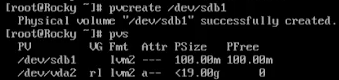
\includegraphics{5.png}
	\end{frame}
\end{enumerate}

\subsection{Создание группы томов и логических томов}
\begin{enumerate}
	\begin{frame}[plain]
		\frametitle{Создание группы томов и логических томов}
		\item В терминале с полномочиями администратора проверьте доступность физических
		томов в вашей системе:
		\item Создайте группу томов с присвоенным ей физическим томом:
		\item Убедитесь, что группа томов была создана успешно:
		\\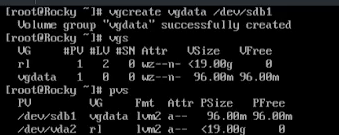
\includegraphics{6.png}
	\end{frame}
	\begin{frame}[plain]
		\item Создайте логический том LVM с именем \texttt{lvdata}, который будет использовать
		50\% доступного дискового пространства в группе томов \texttt{vgdata}:
		\item Проверьте успешность добавления тома:
		\\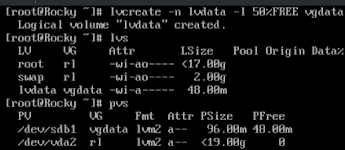
\includegraphics{7.png}
	\end{frame}
	\begin{frame}[plain]
		\item Создайте файловую систему поверх тома:
		\item Создайте директорию, на которую можно смонтировать том:
		\item Добавьте следующую строку в \texttt{/etc/fstab} \texttt{/dev/vgdata/lvdata /mnt/data ext4 defaults 1 2}:
		\item Проверьте, монтируется ли файловая система:
		\\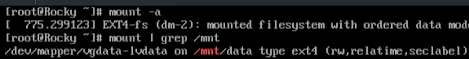
\includegraphics{9.png}
	\end{frame}
\end{enumerate}

\subsection{Изменение размера логических томов}
\begin{enumerate}
	\begin{frame}[plain]
		\frametitle{Изменение размера логических томов}
		\item В терминале с полномочиями администратора введите \texttt{pvs} и \texttt{vgs}, чтобы отобразить
		текущую конфигурацию физических томов и группы томов.
		\item С помощью \texttt{fdisk} добавьте раздел \texttt{/dev/sdb2} размером 100 М. Задайте тип раздела \texttt{8e}:
		\\
\includegraphics{10.png}
	\end{frame}
	\begin{frame}[plain]
		\item Создайте физический том:
		\item Расширьте \texttt{vgdata}:
		\item Проверьте, что размер доступной группы томов увеличен:
		\\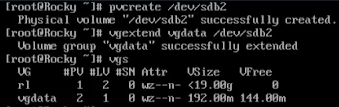
\includegraphics{11.png}
	\end{frame}
	\begin{frame}[plain]
		\item Увеличьте \texttt{lvdata} на 50\% оставшегося доступного дискового пространства в группе томов:
		\item Убедитесь, что добавленное дисковое пространство стало доступным:
		\\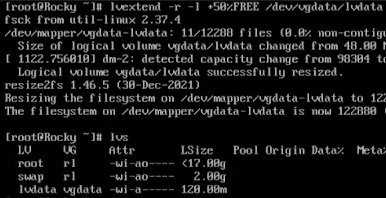
\includegraphics{12.png}
	\end{frame}
	\begin{frame}[plain]
		\item Уменьшите размер \texttt{lvdata} на 50 МБ:
		\item Убедитесь в успешном изменении дискового пространства:
		\\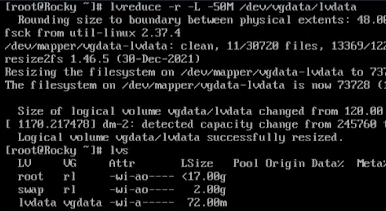
\includegraphics{13.png}
	\end{frame}
\end{enumerate}


\subsection{Самостоятельная работа}
\begin{enumerate}
	\begin{frame}[plain]
		\frametitle{Самостоятельная работа}
		\item Создайте логический том \texttt{lvgroup} размером 200 МБ. Отформатируйте его в
		файловой системе XFS и cмонтируйте его постоянно на \texttt{/mnt/groups}. Перезагрузите
		виртуальную машину, чтобы убедиться, что устройство подключается.
	\end{frame}
	\begin{frame}[plain]
		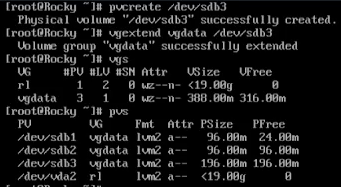
\includegraphics{14.png}
	\end{frame}
	\begin{frame}[plain]
		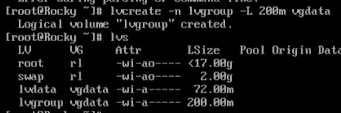
\includegraphics{15.png}
		
\includegraphics{16.png}
		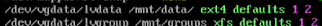
\includegraphics{17.png}
	\end{frame}
	\begin{frame}[plain]
		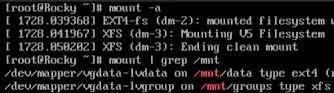
\includegraphics{18.png}
	\end{frame}
	\begin{frame}[plain]
		\item После перезагрузки добавьте ещё 150 МБ к тому \texttt{lvgroup}. Убедитесь, что размер
		файловой системы также изменится при изменении размера тома.
		\\
\includegraphics{19.png}
	\end{frame}
	\begin{frame}[plain]
		\item Убедитесь, что расширение тома выполнено успешно.
		\\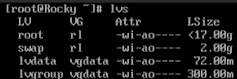
\includegraphics{20.png}
	\end{frame}
\end{enumerate}

\section{Вывод}
\begin{frame}[plain]
	\frametitle{Вывод}
	В ходе выполнения данной работы я получил навыки управления логическими томами.
\end{frame}

\end{document}
